%%%%%%%%%%%%%%%%%%%%%%%%%%%%% Define Article %%%%%%%%%%%%%%%%%%%%%%%%%%%%%%%%%%
\documentclass[xcolor=dvipsnames]{beamer}
\usetheme{presentation}
%%%%%%%%%%%%%%%%%%%%%%%%%%%%% Using Packages %%%%%%%%%%%%%%%%%%%%%%%%%%%%%%%%%%
%\usepackage[cjk]{kotex}
%\usepackage{listings}
\usepackage{tikz}
%%%%%%%%%%%%%%%%%%%%%%%%%%%%%%% Title & Author %%%%%%%%%%%%%%%%%%%%%%%%%%%%%%%%
\title{Causal Inference with Ordinal Outcomes}
\subtitle{Density Estimation Based Approach}
\author{Chanhyuk Park}
\institute{Washington University in St. Louis}
\date{}
%%%%%%%%%%%%%%%%%%%%%%%%%%%%%%%%%%%%%%%%%%%%%%%%%%%%%%%%%%%%%%%%%%%%%%%%%%%%%%%

\begin{document}
   \frame{\titlepage}

\begin{frame}{Motivation}
    \begin{itemize}
        \item Growing emphasis on causal identification in political science
        \item Outcomes are measured in Ordinal scale 
            \begin{itemize}
                \item Approval ratings {\tiny\citep{Canes-Wrone2002a, Kriner2009a}}
                \item Trade policy {\tiny\citep{Scheve2001r, Mayda2005a, Wu2022a}}
            \end{itemize}
        \item The Problem: 
            \begin{itemize}
                \item The usual causal inference tools are designed to serve cardinal or at least interval outcomes
            \end{itemize}
    \end{itemize}
\end{frame}

\begin{frame}{The Goal}
    \begin{itemize}
        \item Treatment effect can only be identified up to scale
            \begin{itemize}[<+->]
                \item ATE resides in the unknown latent space
                \item Consistent normalization may help comparison and interpretation
            \end{itemize}
        \item Flexible density estimation based estimators
            \begin{itemize}[<+->]
                \item Standard parametric approaches rely on strong distributional assumptions, inconsistent
                \item Density estimation techniques can help
            \end{itemize}
    \end{itemize}
\end{frame}

\begin{frame}{Problem Setting}
    \begin{itemize}[<+->]
        \item Suppose a DGP 
            $$
            Y_i^\ast = f(X_i,\beta) + D_i^\top\tau + \varepsilon_i,
            $$
        \item $Y_{i}^{\ast}$ is outcome in unidimensional space that we cannot observe
        \item $D_{i}$ denotes a binary treatment
        \item We only can observe the transformed version of it, $Y_{i} \in \{1, \ldots, j, \ldots, J \}$
            $$
                Y_{i} = \begin{cases}
                    0 & \text{if } \alpha_{-1} < Y_{i}^{\ast} \le \alpha_{0} \\
                    \vdots & \vdots  \\
                    J & \text{if } \alpha_{J-1} < Y_{i}^{\ast} \le \alpha_{J} \\
                \end{cases}
            $$, where $\alpha_{j}$ denotes the threshold points for each ordinal category 
    \end{itemize}
\end{frame}

\begin{frame}{Problem Setting}
    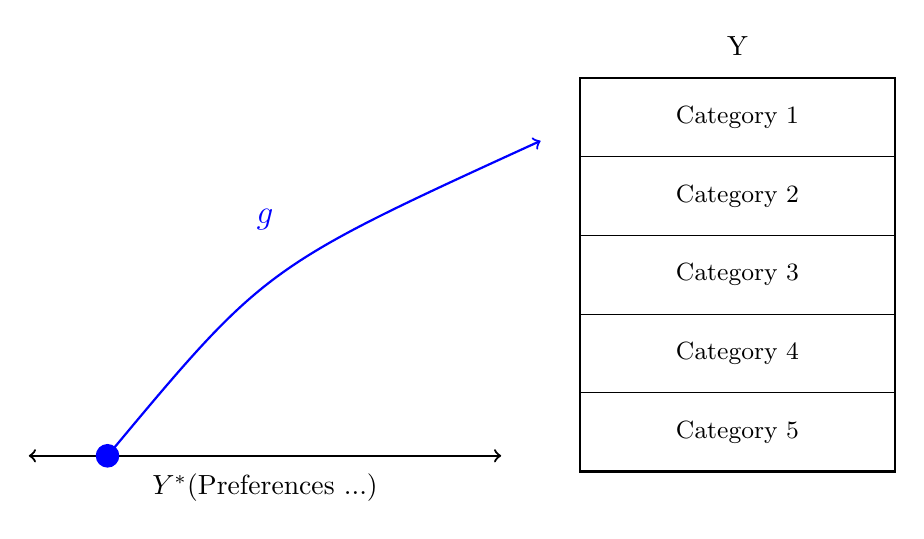
\begin{tikzpicture}
    % Left axis with point and curve
    \draw[thick, <->] (-1,0) -- (5,0);
    \fill[blue] (0,0) circle (0.15cm);
    \draw[blue, thick, ->] (0,0) .. controls (2,2.4) .. (5.5,4);
    \node[blue] at (2,3) {\large $g$};
    \node at (2,-0.4) {$Y^*$(Preferences ...)};

    % Right-hand Y-scale
    \draw[thick] (6,-0.2) rectangle (10.0,4.8);
    \foreach \y in {0.8,1.8,2.8,3.8} { \draw (6,\y) -- (10.0,\y); }

    \node at (8,4.3) {\small Category 1};
    \node at (8,3.3) {\small Category 2};
    \node at (8,2.3) {\small Category 3};
    \node at (8,1.3) {\small Category 4};
    \node at (8,0.3) {\small Category 5};

    \node at (8,5.2) {Y};
    \end{tikzpicture}
\end{frame}

\begin{frame}{Potential Outcome Framework}
    \begin{itemize}[<+->]
        \item Denote the binary treatment status of individual $D_{i} \in \{0, 1\}$
        \item Denote the potential outcomes in latent preference scale as $Y_{i}^{\ast}(D_{i})$
            \begin{itemize}
                \item $Y_{i}^{\ast}(1) = \tau + f(\beta, X_{i}) + \epsilon_{i}$
                \item $Y_{i}^{\ast}(0) = f(\beta, X_{i}) + \epsilon_{i}$
            \end{itemize}
        \item Denote the potential outcomes in observed ordinal scale (POO) as $Y_{i}(d_{i}) = g(Y_{i}^{\ast}(d_{i})) \in \{1, \ldots, j,\ldots J\}$
        \item We are interested in the average treatment effect in the latent space (LTE)
            $$
            \begin{aligned}
                LTE &= \mathbb{E}\left[Y^{\ast}(1)\right] - \mathbb{E}\left[Y^{\ast}(0)\right] \\
                &= \tau
            \end{aligned}
            $$ 
    \end{itemize}
\end{frame}

\begin{frame}{LTE with $Y_{i}(D_{i})$}
\begin{itemize}
    \item If $Y_{i}^{\ast}$ is known, there is not problem
    \item If $g$ is known and it maps one value of $Y_{i}^{\ast}$ to $Y_{i}$, then we may get LTE, but this not true in most settings
        $$
            \mathbb{E}\left[g^{-1}(Y_{i}(1))\right] - \mathbb{E}\left[g^{-1}(Y_{i}(0))\right] \neq LTE
        $$ 
    \item Should we give up?
\end{itemize}
\end{frame}

\begin{frame}{Up To Scale Identification}
    \begin{itemize}[<+->]
        \item We can identify LTE up to scale (Theorem 1)
        \item From the model and data we know:
            $$
            \begin{aligned}
                \mathbb{P}\left(Y(D) \le j\right) &= \mathbb{P}\left(Y^{\ast} \le \alpha_j \right) \\
            \end{aligned}
            $$  
        \item We can construct MLE with using this probability.
        \item However, if we scale $Y^{\ast}$ side by a constant, $c > 0$, we still get the same probability
            $$
            \begin{aligned}
                \mathbb{P}\left(Y(D) \le j\right) &= \mathbb{P}\left(Y^{\ast} \le \alpha_j \right) \\
                &= \mathbb{P}\left(c Y^{\ast} \le c \alpha_j\right) \\
            \end{aligned}
            $$  
    \end{itemize}
\end{frame}

\begin{frame}{Normalization}
    \begin{itemize}[<+->]
        \item Up to scale identification is disappointing
        \item Proper normalization helps interpretation and comparison across models and across samples
        \item Fixing $Var(\varepsilon_{i}) = 1$ is one way
        \item This works as mapping $Y_{i}^{\ast}$ to the space where the variance of the error is a unit / probit space
    \end{itemize}
\end{frame}

\begin{frame}{Common Transformation: Cardinalization and Binarization}
    \begin{itemize}
        \item Cardinalization
            \begin{itemize}
                \item Relies on luck
            \end{itemize}
        \item Binarization
            \begin{itemize}
                \item Lose significant efficiency
                \item Estimate may be sensitive to how you group the ordinal outcomes
            \end{itemize}
    \end{itemize}
\end{frame}

\begin{frame}{Small Example}
    \begin{table}[ht]
        \centering
        \begin{tabular}{c|cc}
            \hline
             & $Y_i^\ast(0)$ & $Y_i^\ast(1)$ \\
            \hline
            A &  1.37 & 0.09 \\
            B & -0.56 & 1.71 \\
            C &  0.36 & 0.11 \\
            D &  0.63 & 2.22 \\
            E &  0.40 & 0.14 \\
            \hline
        \end{tabular}
        \label{tab:latent_example}
    \end{table}
    \begin{itemize}
        \item The LTE in the latent preference space is: $0.41$
    \end{itemize}
\end{frame}

\begin{frame}{Small Example -- Cardinalization}
    \begin{itemize}
        \item Suppose two transformation functions: $g_{a}$ and $g_{b}$
        \item Both are monotone, but with different thresholds ($\alpha_{j}$)
    \end{itemize}
    \begin{table}[ht]
        \centering
        \begin{tabular}{c|cc|cc}
            \hline
            & \multicolumn{2}{c|}{$g_a$} & \multicolumn{2}{c}{$g_b$} \\
            & $Y_{i,g_a}(0)$ & $Y_{i,g_a}(1)$ & $Y_{i,g_b}(0)$ & $Y_{i,g_b}(1)$ \\
            \hline
            A & Agree          & Agree          & Agree          & Disagree \\
            B & Neither        & Agree          & Disagree       & Agree    \\
            C & Agree          & Agree          & Neither        & Disagree \\
            D & Agree          & Strongly Agree & Neither        & Agree    \\
            E & Agree          & Agree          & Neither        & Disagree \\
            \hline
        \end{tabular}
        \label{tab:g_example}
    \end{table}
\end{frame}

\begin{frame}{Small Example -- Cardinalization}
    \begin{itemize}
        \item A researcher impose common cardinalization of 1 to 5,
        \item In case the true transformation is $g_{a}$, the estimate is $-0.4$
        \item In case the true transformation is $g_{b}$, the estimate is $0.2$
        \item Without compelling reason to impose such numeric labels, cardinalization relies on pure luck
    \end{itemize}
\end{frame}

\begin{frame}{Estimation}
    \begin{itemize}
        \item There has been tools for ordinal outcomes
        \item Standard parametric approaches such as Ordered Probit and Ordered Logit
        \item Two estimators based on density estimation techniques
    \end{itemize}
\end{frame}

\begin{frame}{Ordered Logit and Probit}
    \begin{itemize}
        \item Assume that the error term follows a specific distribution (Logistic and Standard Normal)
        \item And use maximum likelihood to estimate the coefficients
        \item Identify coefficients up to scale
        \item Once distributional assumption is violated, inconsistent
    \end{itemize}
\end{frame}

\begin{frame}{Ordered Logit and Probit}
\begin{itemize}
    \item The true log-likelihood is:

    \[
    \begin{aligned}
    \ell(\alpha,\beta,\tau)
    =\;
    &\sum_{i=1}^n \sum_{j=0}^J  
        1_{\{Y_i = j\}}
        \Bigg\{
            \log F\!\left(
                \alpha_j 
                - f(X_i,\beta)
                + D_i^\top \tau
            \right)
    \\
    &\qquad\qquad\qquad
            -\;
            \log F\!\left(
                \alpha_{j-1}
                - f(X_i,\beta)
                + D_i^\top \tau
            \right)
        \Bigg\}
    \end{aligned}
    \]

    \item $F$ is the CDF of the true error.
    \item If $F$ is not standard normal or standard logistic, MLE is inconsistent.
    \item The error is never known, and omitted or unobserved confounder may also distort the error
\end{itemize}
\end{frame}

\begin{frame}{Alternative: Estimate the $F$}
    \begin{itemize}
        \item Instead of assuming a specific $F$, we can estimate as $\hat{F}$
        \item Then the log-likelihood becomes:
            \[
            \begin{aligned}
                \hat{\ell}(\alpha,\beta,\tau)
            =\;
            &\sum_{i=1}^n \sum_{j=0}^J  
                1_{\{Y_i = j\}}
                \Bigg\{
                    \log \hat{F}\!\left(
                        \alpha_j 
                        - f(X_i,\beta)
                        + D_i^\top \tau
                    \right)
            \\
            &\qquad\qquad\qquad
                    -\;
                    \log \hat{F}\!\left(
                        \alpha_{j-1}
                        - f(X_i,\beta)
                        + D_i^\top \tau
                    \right)
                \Bigg\}
            \end{aligned}
            \]
        \item I propose to use two density estimation methods: KDE and Normalizing Flows
    \end{itemize}
\end{frame}

\begin{frame}{Kernel Density Estimation}
    \begin{itemize}
        \item Nonparametric method
        \item Smooth each observation using a kernel (usually Gaussian)
            $$
                \hat f(x)
= \frac{1}{n h} \sum_{i=1}^n K\!\left( \frac{x - X_i}{h} \right)
            $$ 
        \item Generally, the moderate bandwidth ensures enough convergence rate for $\sqrt{n}$ consistency for the main estimator (semiparametric efficiency)
    \end{itemize}
\end{frame}

\begin{frame}{Normalizing Flows}
    \begin{itemize}
        \item A flexible class of models that transform complex continuous density to simple base density (usually Gaussian)
        \item Use the change-of-variable formula
            $$
                f_\theta(h)
                = f_Z\bigl(T_\theta^{-1}(h)\bigr)
                \left|\det \D T_\theta^{-1}(h)\right|,
            $$
        \item $T_{\theta}$ is a set of \textit{invertible} transformation
        \item Rational Quadratic Spline Flow
        \item Since this is fully parametric, for finite $\theta$, MLE ensures $\sqrt{n}$ consistency
    \end{itemize}
\end{frame}

\begin{frame}{Simulation}
    \begin{itemize}
        \item Ordered Probit Ordered Logit and NF based only
        \item Errors: Standard Normal and Log Normal distribution
        \item A binary treatment randomized 
        \item Covariates: One binary and three continuous (following normal distribution)
        \item Thresholds: $-2, -1, 1, 2.5$ $\rightarrow$ 5 categories
        \item Sample sizes: 200, 500, 1000, 2000
        \item 200 Replications
    \end{itemize}
\end{frame}

\begin{frame}{Simulation}
\begin{figure}
    \begin{tabular}{cc}
        \includegraphics[width=0.45\textwidth]{../figures/latent_space_normal_N1000000.png} & \includegraphics[width=0.45\textwidth]{../figures/latent_space_lognormal_N1000000.png}\\
    \end{tabular}
\end{figure}
\end{frame}

\begin{frame}{Simulation -- Normal Case}
    \begin{itemize}
        \item True treatment size: 1.0
    \end{itemize}
\begin{figure}
    \begin{tabular}{cc}
        \includegraphics[width=0.45\textwidth]{../figures/bias_oprobit_ologit_flow_normal.pdf} & \includegraphics[width=0.45\textwidth]{../figures/rmse_oprobit_ologit_flow_normal.pdf}\\
    \end{tabular}
\end{figure}
\end{frame}

\begin{frame}{Simulation -- Lognormal Case}
    \begin{itemize}
        \item True treatment size: 0.46
    \end{itemize}
\begin{figure}
    \begin{tabular}{cc}
        \includegraphics[width=0.45\textwidth]{../figures/bias_oprobit_ologit_flow_lognormal.pdf} & \includegraphics[width=0.45\textwidth]{../figures/rmse_oprobit_ologit_flow_lognormal.pdf}\\
    \end{tabular}
\end{figure}
\end{frame}

\begin{frame}{Conclusion}
    \begin{itemize}
        \item With ordinal outcomes, treatment effects can only be identified up to scale
        \item Cardinalization and Binarization have its pitfalls
        \item Standard parametric approaches relies on strong distributional assumption
        \item KDE and NF based approaches may provide flexible ways to estimate the true effects
        \item For KDE, the normalization of coefficients is an issue...
        \item For NF, Hyperparameter selection is an issue, trying to automatically adjust it while traing
    \end{itemize}
\end{frame}

\end{document}
